%%%%%%%%%%%%%%%%%%%%%%%%%%%%%%%%%%%%%%%%%%%%%%%%%%%%%%
% A Beamer template for Ritsumeikan University       %
% Author: Ming-Hao Xu (Xu Minghao)                   %
% Date:   April 2022.                                %
% LPPL Licensed.                                     %
%%%%%%%%%%%%%%%%%%%%%%%%%%%%%%%%%%%%%%%%%%%%%%%%%%%%%%

\documentclass[10pt]{beamer}
\usepackage{hyperref}

\usepackage[UTF8]{ctex}
\usepackage[T1]{fontenc}
\usepackage[backend=bibtex]{biblatex}
\addbibresource{ref.bib}

% other packages
\usepackage{latexsym,amsmath,xcolor,multicol,booktabs,calligra}
\usepackage{graphicx,pstricks,listings,stackengine}
\usefonttheme[onlymath]{serif}

% dummy text; remove it when working on this template
\usepackage{lipsum}

\setbeamerfont{footnote}{size=\tiny}

\author{Wenchong Huang}
\title{Adaptive Mesh Refinement Design}
\institute{
    School of Mathematical Sciences, \\
    Zhejiang University.
}
\date{Mar. 8th, 2024}
\usepackage{Ritsumeikan}

% defs
\def\cmd#1{\texttt{\color{red}\footnotesize $\backslash$#1}}
\def\env#1{\texttt{\color{blue}\footnotesize #1}}
\definecolor{deepblue}{rgb}{0,0,0.5}
\definecolor{deepred}{rgb}{0.6,0,0}
\definecolor{deepgreen}{rgb}{0,0.5,0}
\definecolor{halfgray}{gray}{0.55}

\lstset{
    basicstyle=\ttfamily\tiny,
    keywordstyle=\bfseries\color{deepblue},
    emphstyle=\ttfamily\color{deepred},    % Custom highlighting style
    stringstyle=\color{deepgreen},
    numbers=left,
    numberstyle=\small\color{halfgray},
    rulesepcolor=\color{red!20!green!20!blue!20},
    frame=shadowbox,
}


\begin{document}

\begin{frame}
    \titlepage
\end{frame}

\section{任务简介}

\begin{frame}[fragile]{研究背景}
    \footnotesize

    \begin{figure}[H]
        \centering
        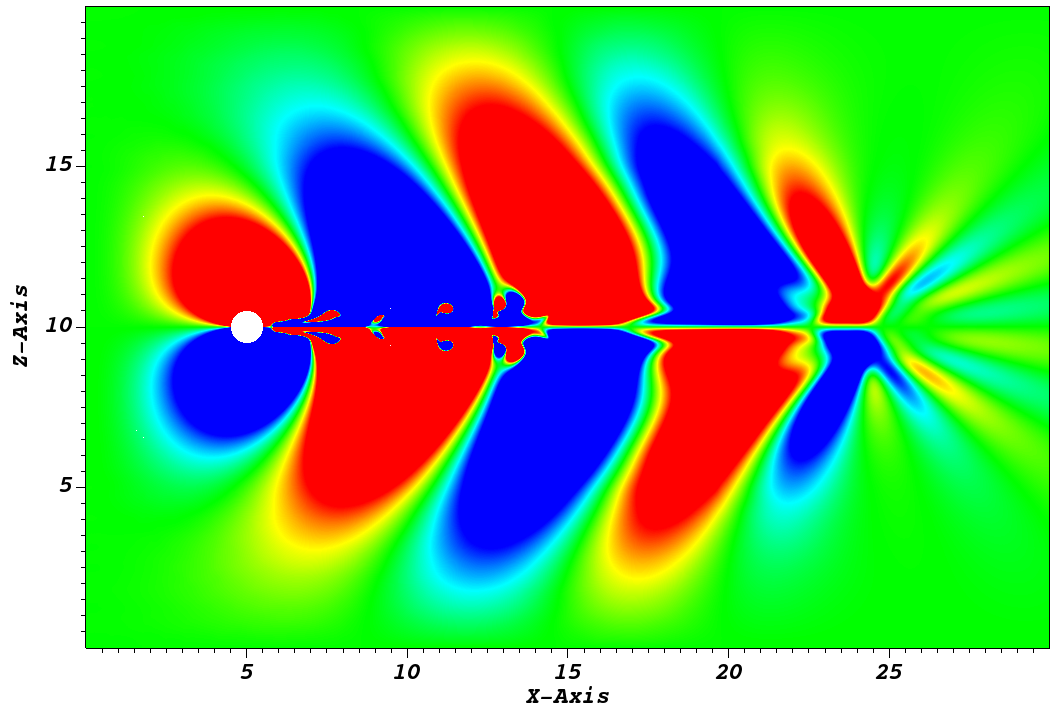
\includegraphics[width=0.3\textwidth]{png/densityPerturbation.png}
        \caption{\footnotesize 在密度分层流体中小球拖曳造成的密度扰动.}
    \end{figure}

    \vspace{-1em}

    \begin{figure}[H]
        \centering
        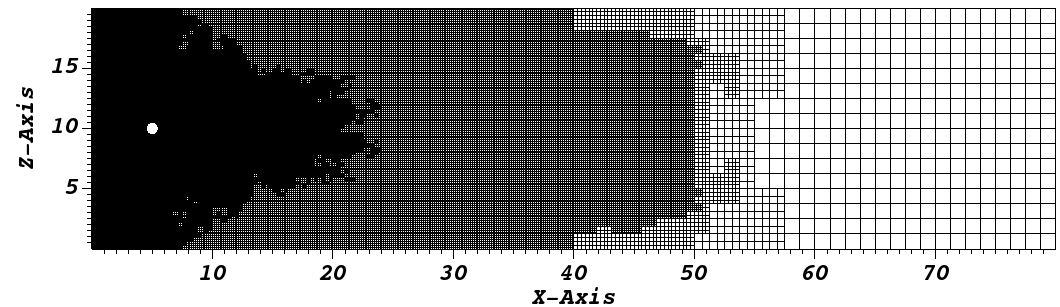
\includegraphics[width=0.8\textwidth]{png/amrdealii.png}
        \caption{\footnotesize Li 等人用 deal.ii 计算小球拖曳问题时使用的网格 (某特定时刻).}
    \end{figure}

    \vspace{-1em}

    捕捉尾涡要非常细的网格,但全局用这么细的网格跑不动,加并行也没用。
    组里的代码目前不支持自适应,我们要解决这个问题。
\end{frame}

\begin{frame}[fragile]{树形结构的 AMR}
    \footnotesize

    deal.ii 的 AMR 实现基于树形结构.
    \begin{figure}[H]
        \centering
        \begin{minipage}[t]{0.25\textwidth}
            \centering
            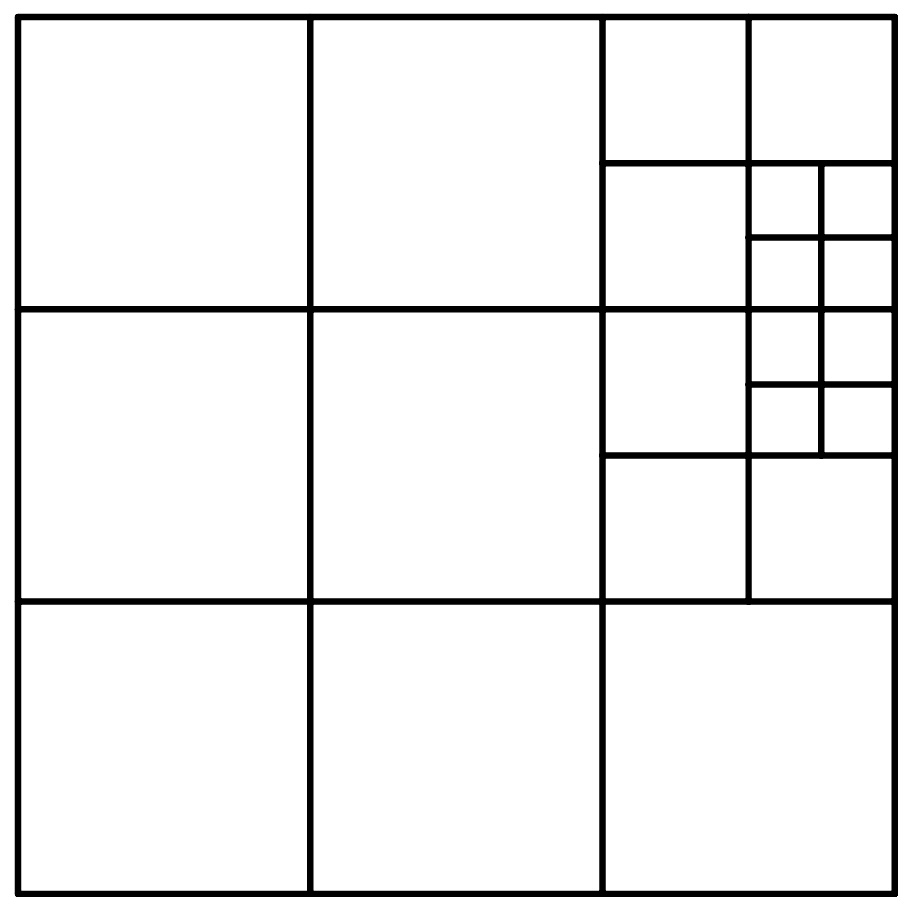
\includegraphics[width=0.95\textwidth]{jpg/treeAMR.jpg}
            \caption{\footnotesize 结构化 AMR}
        \end{minipage}
        \hspace{1em}
        \begin{minipage}[t]{0.6\textwidth}
            \centering
            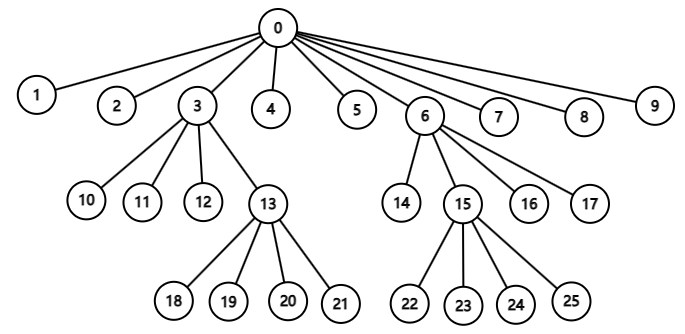
\includegraphics[width=0.85\textwidth]{png/treeStorge.png}
            \caption{\footnotesize 存储左图所示 AMR 的树形数据结构}
        \end{minipage}
    \end{figure}

    \pause
    树形数据结构内存不连续, 内存索引将会增加大量耗时.
\end{frame}

\begin{frame}[fragile]{块状加密的 AMR}
    \footnotesize

    上世纪 90 年代, 美国 Lawrence Berkeley 国家实验室
    开发了一套支持基于块状加密的 AMR 网格与并行计算
    的基础软件设施库 Chombo\footfullcite{ChomboDesign} \footfullcite{ChomboAMR} . 

    \begin{figure}[H]
        \centering
        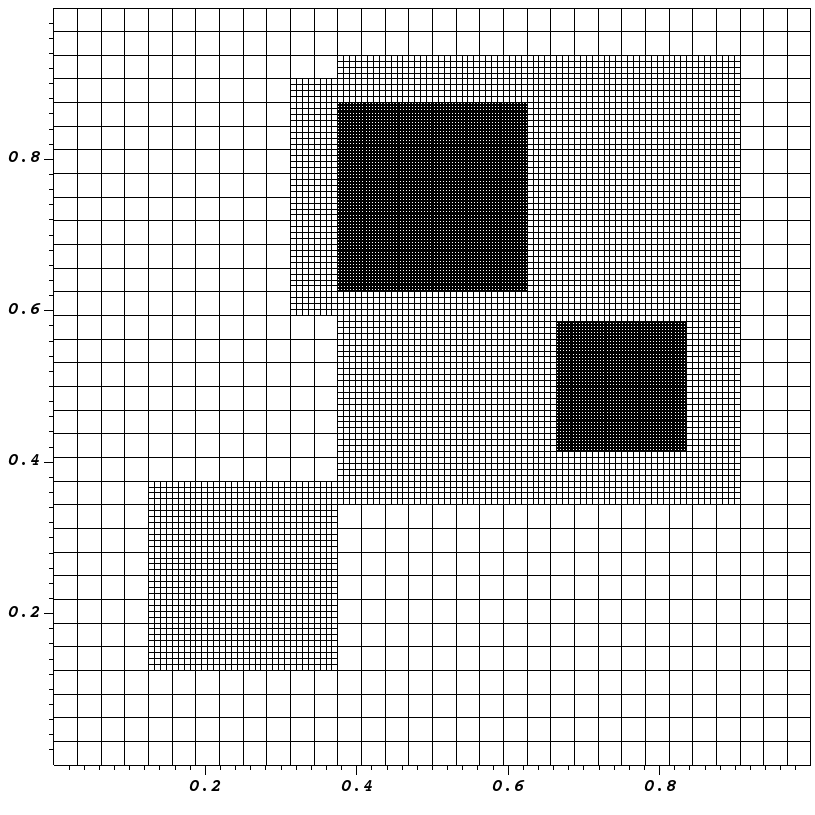
\includegraphics[width=0.3\textwidth]{png/blockAMR.png}
        \caption{\footnotesize 基于块状加密的 AMR 示意图.}
    \end{figure}

    \vspace{-1.2em}
    用户可以选择物理区域中的若干个块状区域进行加密,
    每一个加密块在内存中都是连续的.
    用户还可以自定义加密率.

    \pause
    但是, Chombo 的代码实现过于老旧, 
    不符合现代编程理念.
    另外, 它将不规则边界当成一段一段的线段 \footfullcite{ChomboEmbeddedBoundary},
    这导致它在不规则区域中不能做到高阶精度.
\end{frame}

\section{前人的工作}

\begin{frame}[fragile]{DisjointBoxLayout (done by Qian et al.)}
    \footnotesize
    用一个 \verb|DisjointBoxLayout| 封装同一层级的
    的所有块状加密区域,每个区域是一个 \verb|Box|.
    用 \verb|std::vector<DisjointBoxLayout>| 来存储整个 AMR 网格.

    \begin{figure}[H]
        \centering
        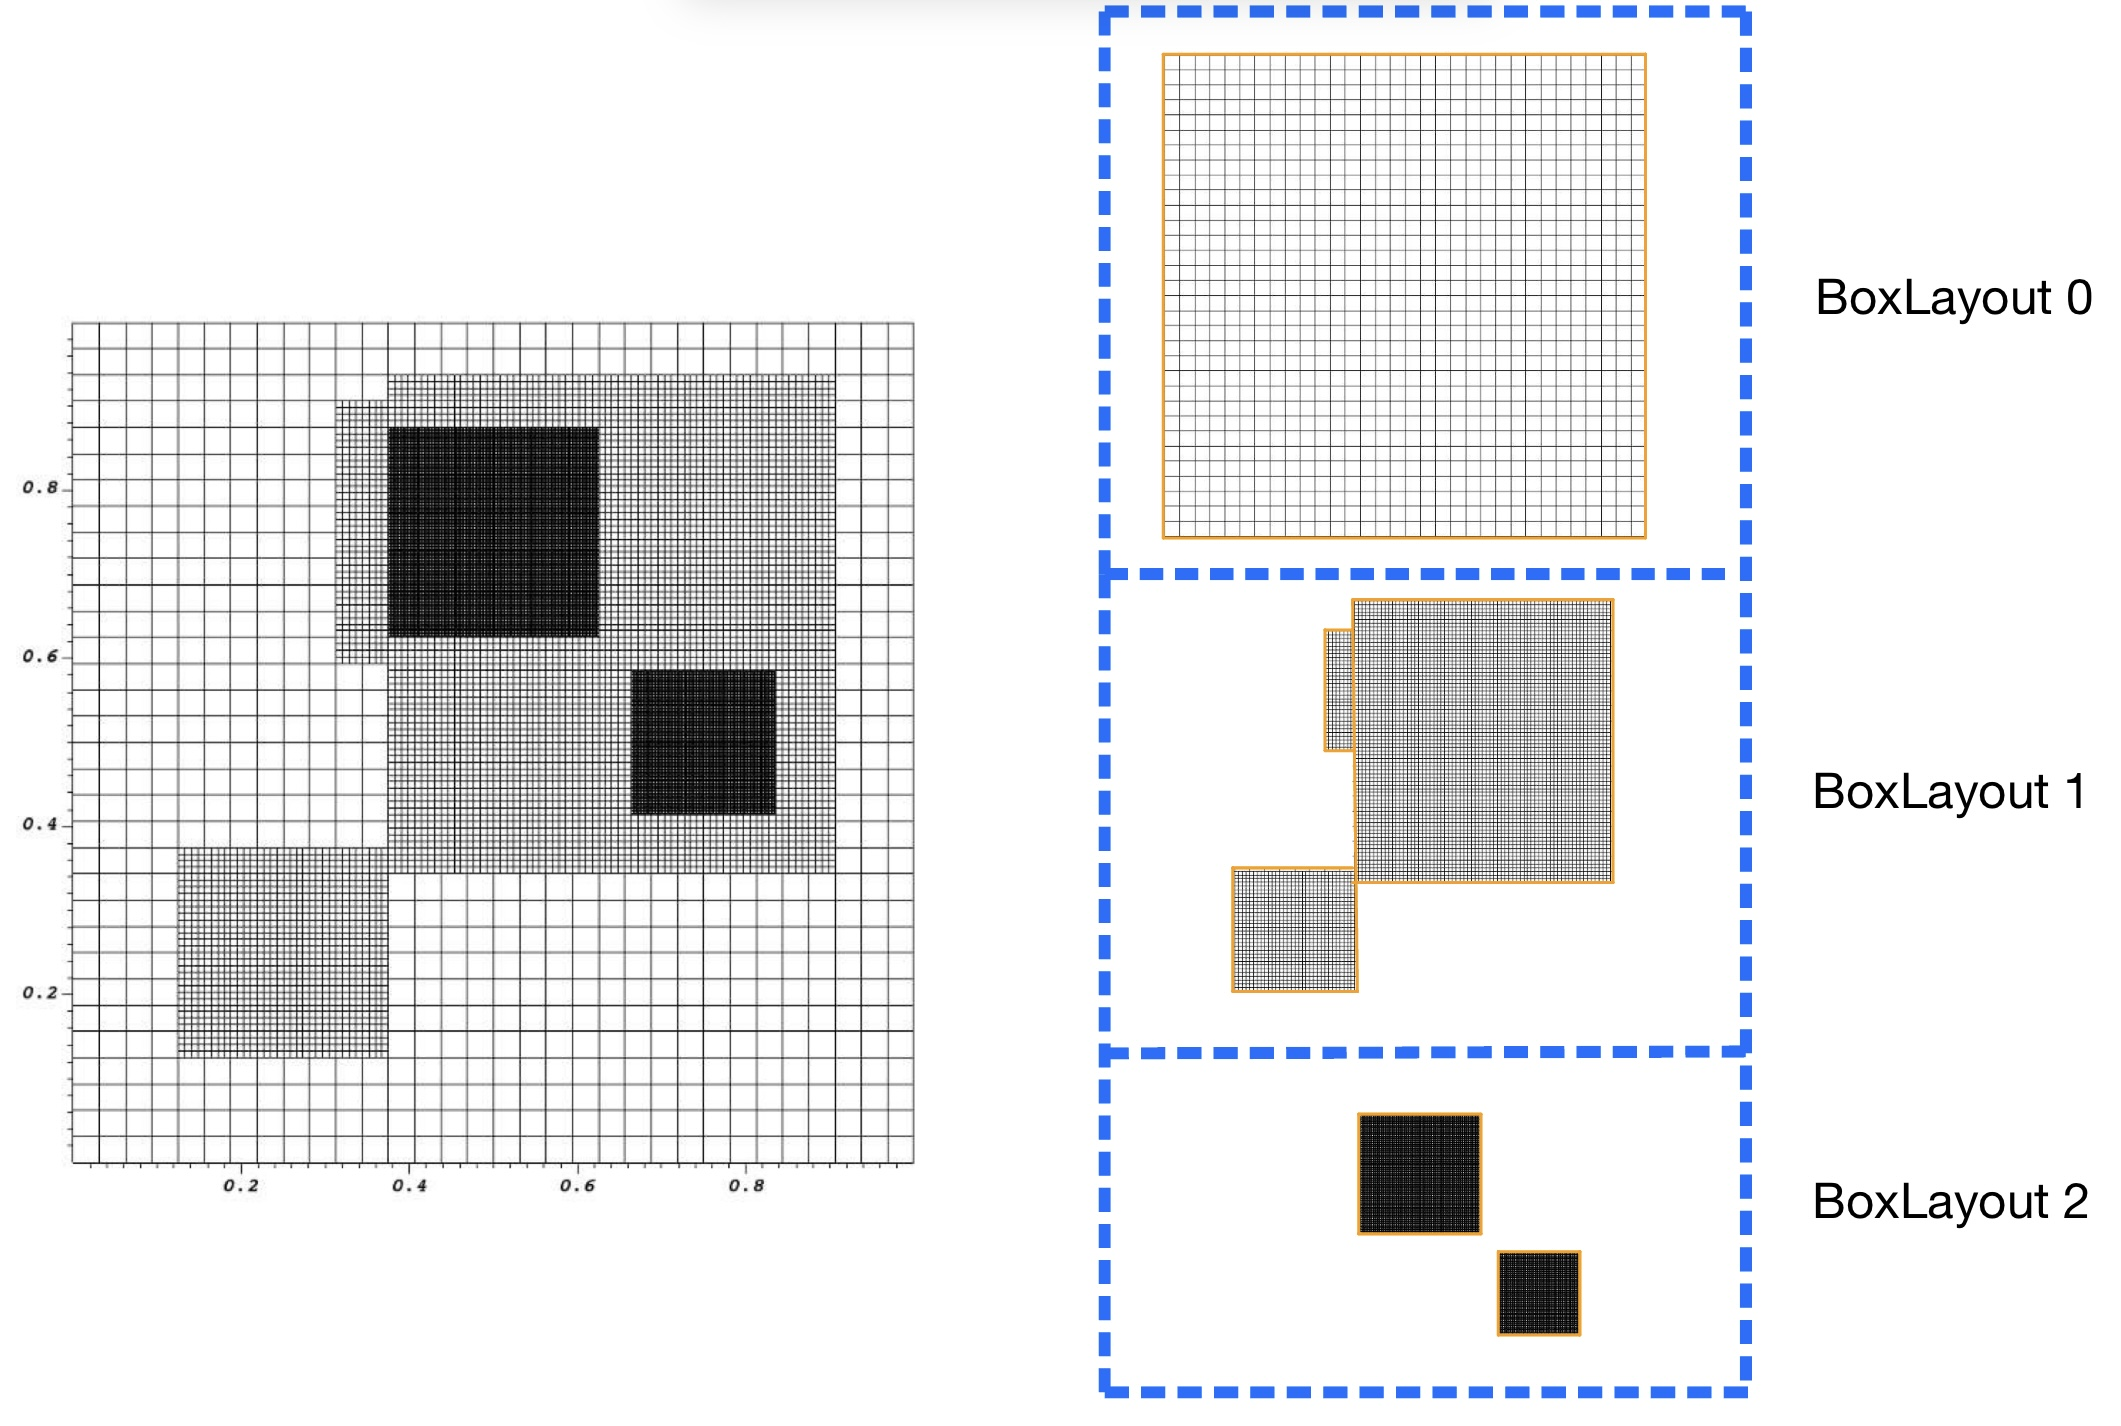
\includegraphics[width=0.7\textwidth]{jpg/BoxLayout.jpeg}
    \end{figure}

    用户可以指定每个 \verb|Box| 由几号线程来处理。
\end{frame}

\begin{frame}[fragile]{LevelData (done by Qian et al.)}
    \footnotesize
    \verb|LevelData| 与 \verb|DisjointBoxLayout| 关联,
    每个 \verb|Box| 的数据存储在一个 \verb|Tensor| 里,
    用一个 \verb|std::vector<Tensor>| 存储
    所有由当前线程处理的 \verb|Box| 中的数据.

    \begin{figure}[H]
        \centering
        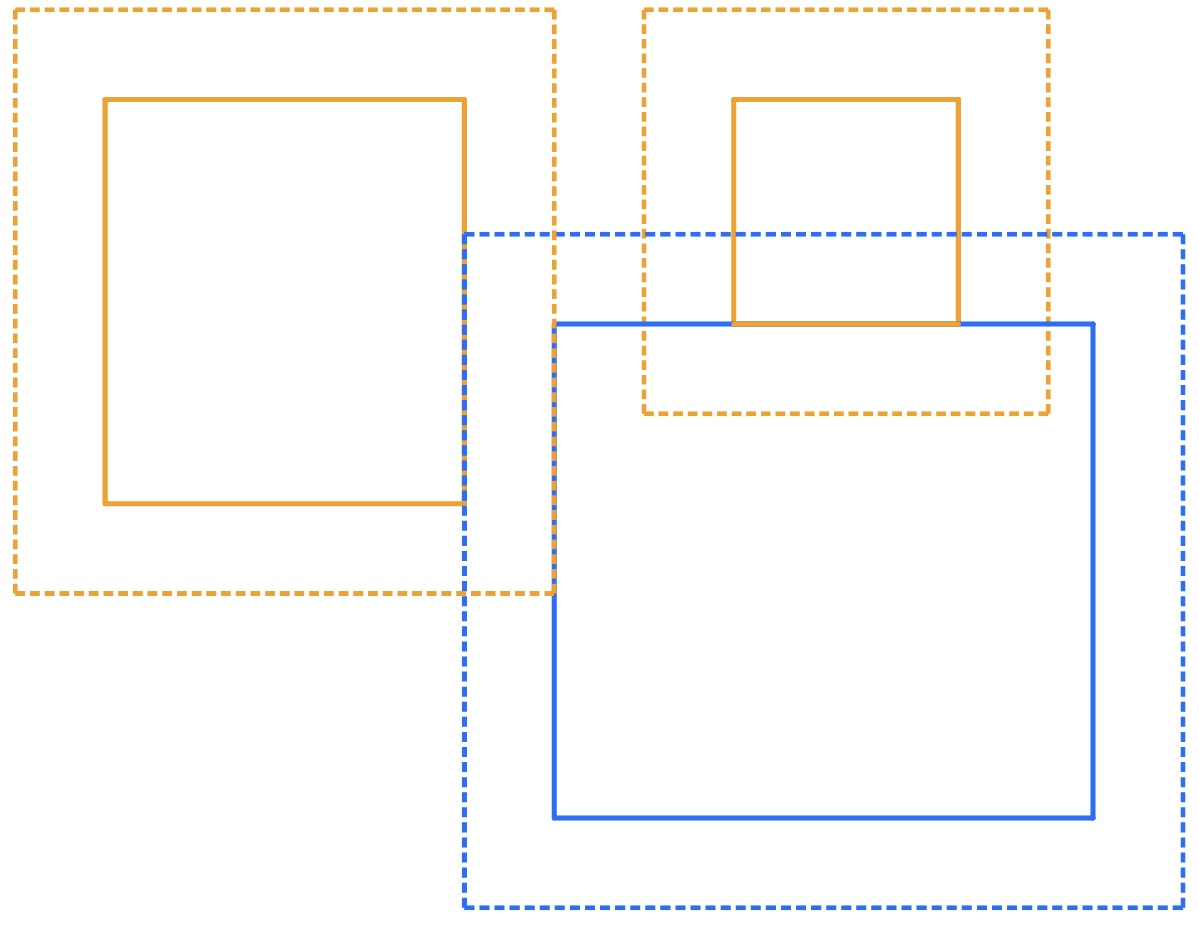
\includegraphics[width=0.7\textwidth]{jpg/LevelData.jpeg}
        \caption{\footnotesize 不同的颜色表示不同线程中的 LevelData 存储的数据, 虚线表示 Ghost Cell.}
    \end{figure}
\end{frame}

\begin{frame}[fragile]{LevelOp}
    \footnotesize
    \verb|LevelOp| 用于对 \verb|LevelData| 做标准四阶离散格式的计算, 
    比如 $\Delta, \nabla, \text{div}$ 等.
    还支持方程 $\alpha\phi+\beta\Delta\phi=f$ 的标准格式 Jacobi 迭代.

    \vspace{1em}
    前提是 \verb|LevelData| 中所有数据以及 Ghost Cell 中的数据均已知.
\end{frame}

\begin{frame}[fragile]{SpatialOp}
    \footnotesize
    \verb|SpatialOperator| 及其派生类
    用于对 \verb|LevelData| 做四阶离散格式的计算, 
    以边界嵌入的方式处理不规则区域.

    \vspace{1em}
    前提是 \verb|LevelData| 中所有数据以及 Ghost Cell 中的数据均已知.
\end{frame}

\begin{frame}[fragile]{多重网格 (V-Cycle)}
    \footnotesize
    \begin{figure}[H]
        \centering
        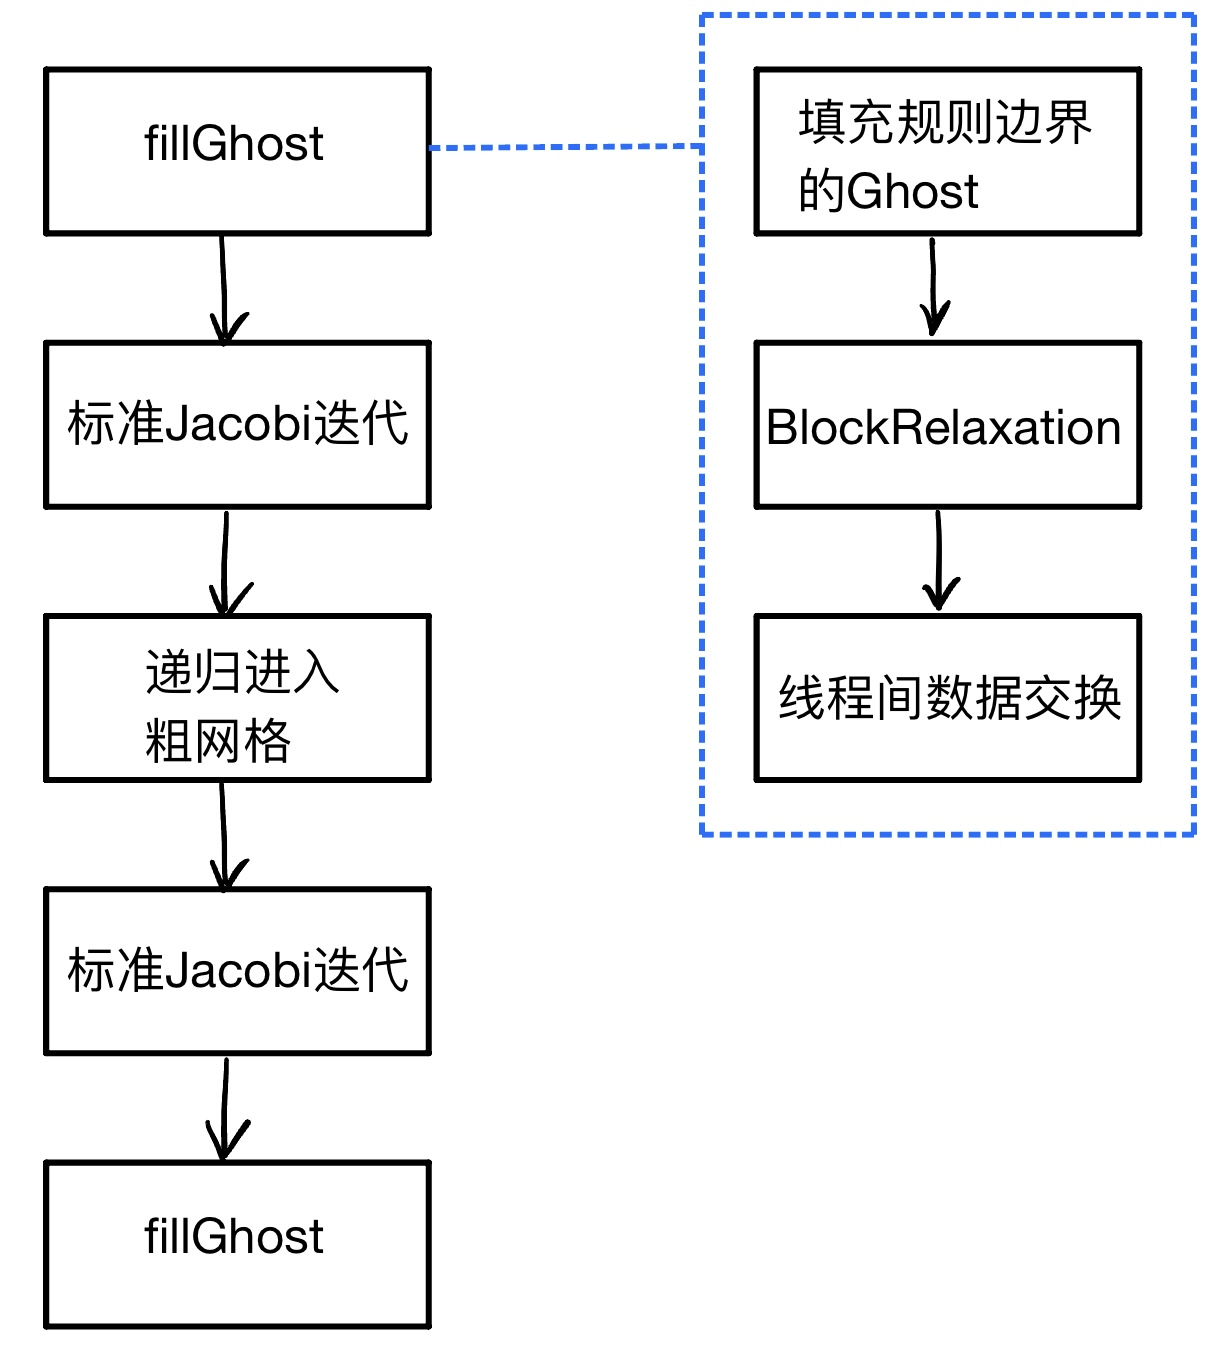
\includegraphics[width=0.5\textwidth]{jpg/v-cycle.jpeg}
        \caption{\footnotesize 不规则区域的多重网格V-Cycle算法.}
    \end{figure}
\end{frame}

\begin{frame}[fragile]{负载均衡器 (done by Qian et al.)}
    \footnotesize
    我们现有的 \verb|LoadBalancer| 可以做到输入一个
    包含嵌入边界的 \verb|Box| 区域,
    程序将区域尽可能均匀地划分,
    然后输出一个 \verb|DisjointBoxLayout|, 
    并为每个新 \verb|Box| 分配线程号.

    \begin{figure}[H]
        \centering
        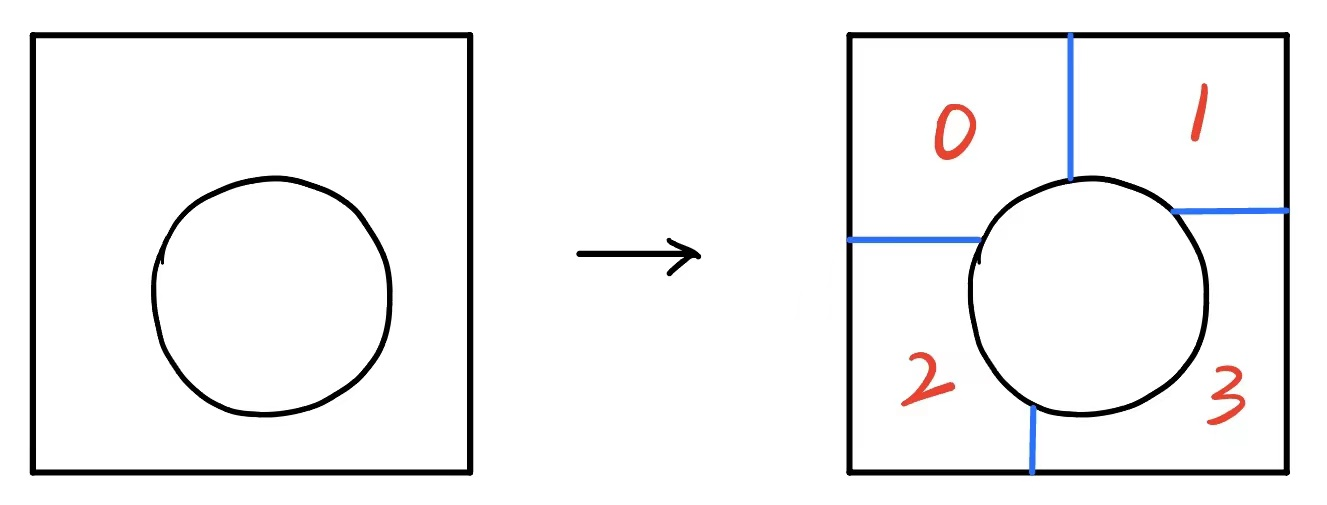
\includegraphics[width=0.8\textwidth]{jpg/oldbalance.jpeg}
        \caption{\footnotesize 负载均衡示意图.}
    \end{figure}
\end{frame}

\section{我们需要完成的任务}

\begin{frame}[fragile]{整体安排}
    \footnotesize

    \begin{figure}[H]
        \centering
        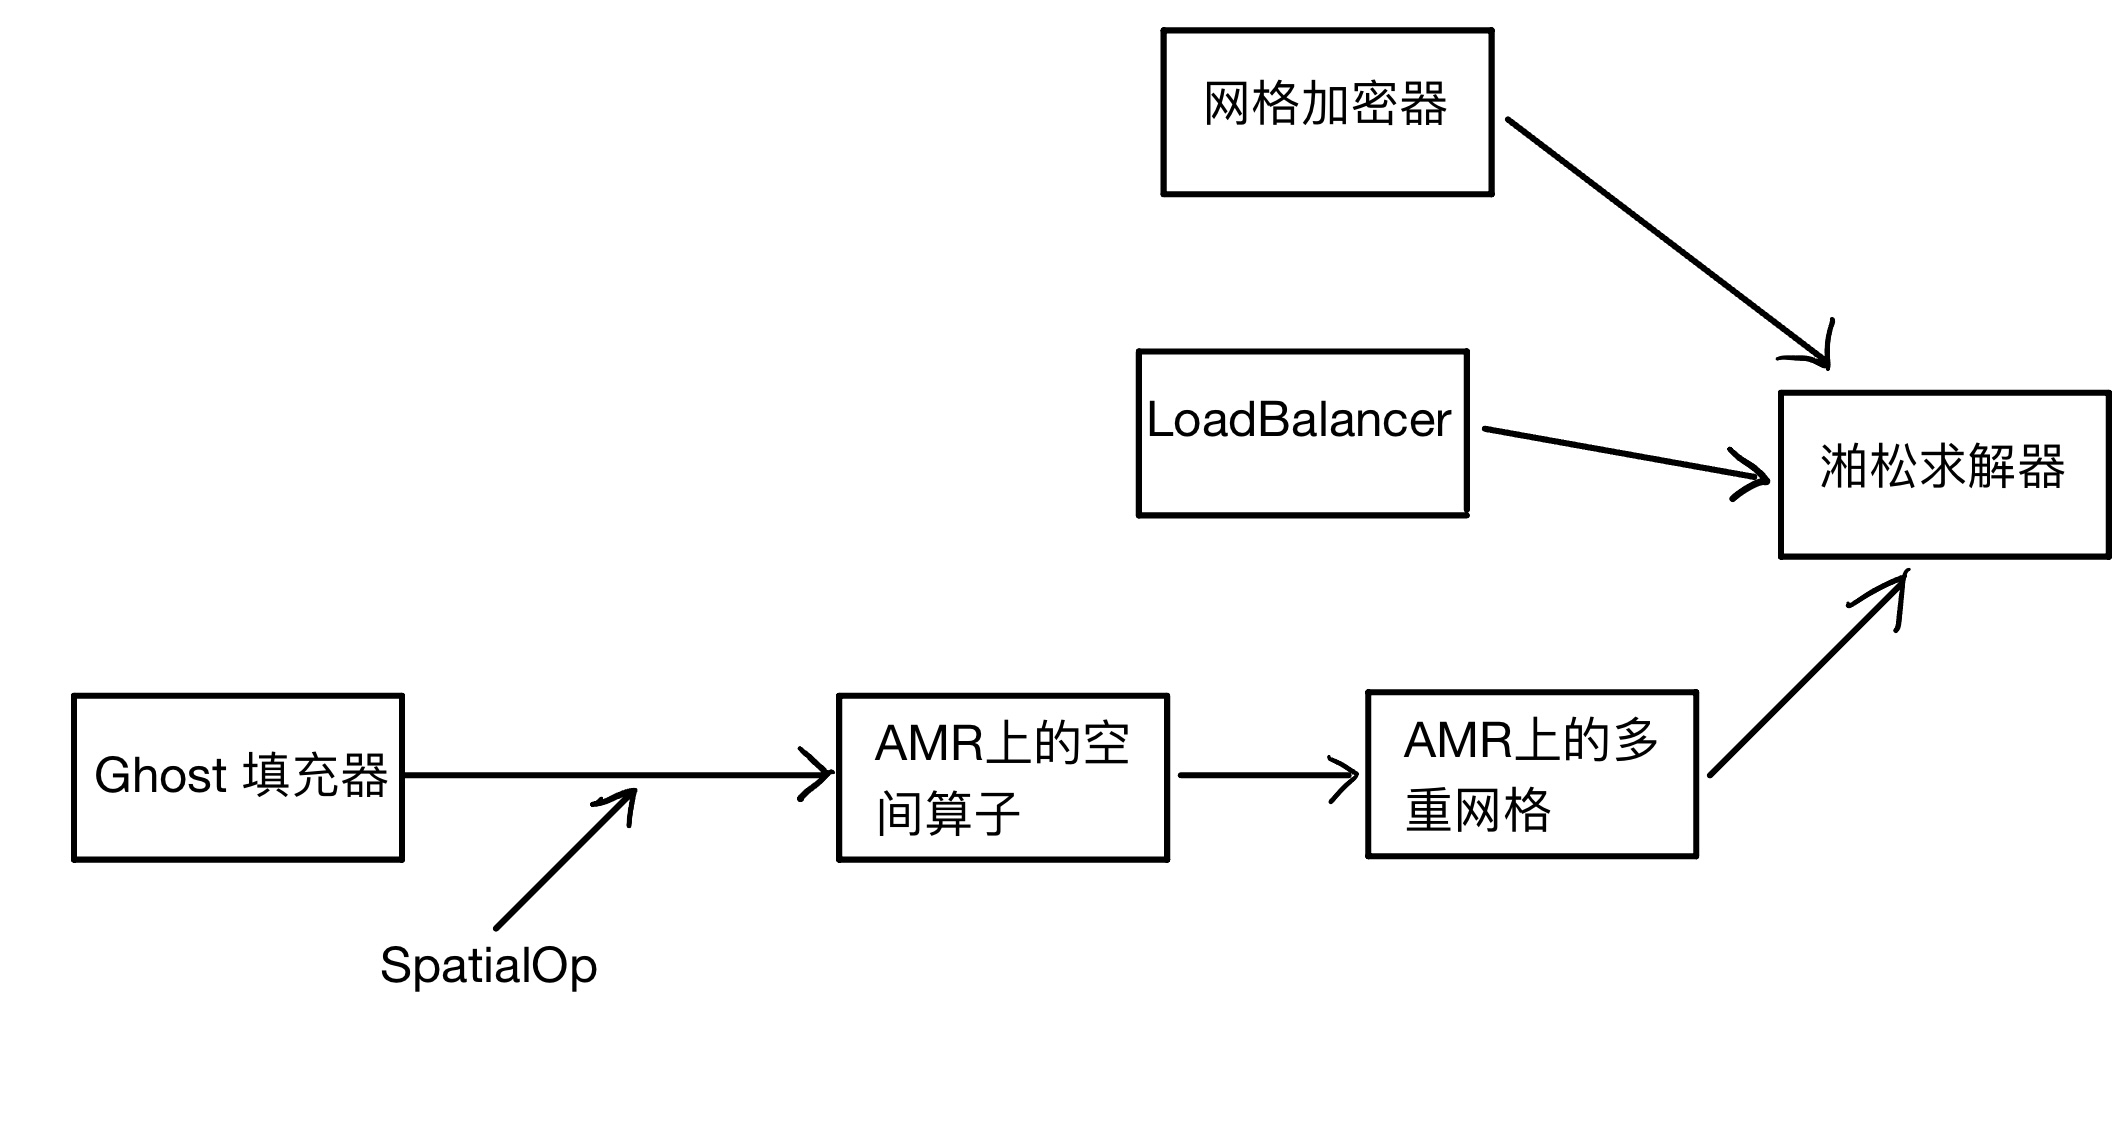
\includegraphics[width=0.8\textwidth]{jpg/plan.jpeg}
        \caption{\footnotesize 任务安排.}
    \end{figure}
\end{frame}

\begin{frame}[fragile]{网格加密}
    \footnotesize

    用一个 \verb|std::vector<LevelData>| 来存储用户标记的需要加密的网格,
    我们根据标记把加密区域处理为块状区域, 兼顾自适应性能和内存访问效率.

    \begin{figure}[H]
        \centering
        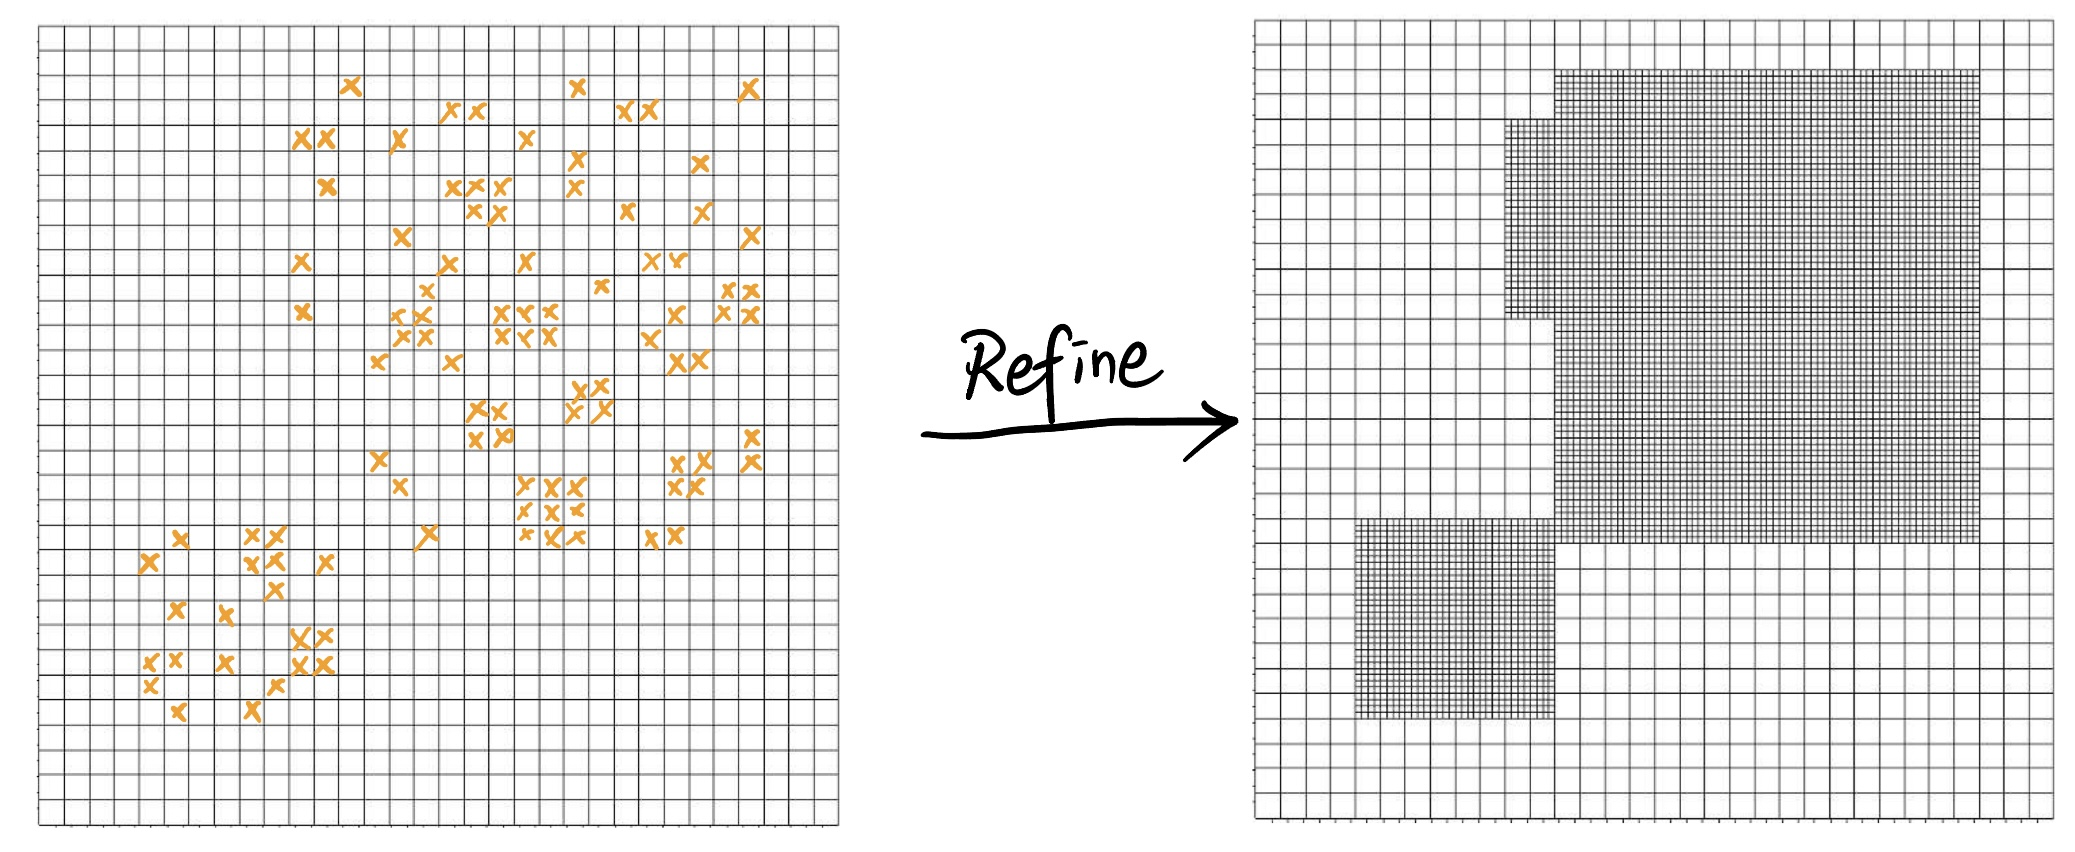
\includegraphics[width=0.8\textwidth]{jpg/refine.jpeg}
        \caption{\footnotesize 块状加密示意图.}
    \end{figure}

    这个功能做一个网格加密器类, 命名为 \verb|BRMeshRefine|.
\end{frame}

\begin{frame}[fragile]{负载均衡器}
    \footnotesize
    当我们同时存在分辨率不同的多个 \verb|Box| 时,
    现有的负载均衡器无法直接使用.
    换言之, 我们现在的输入是 \verb|std::vector<DisjointBoxLayout>|.
    我们仍然希望负载均衡, 且必要时对输入的 \verb|Box| 进一步划分.

    \begin{figure}[H]
        \centering
        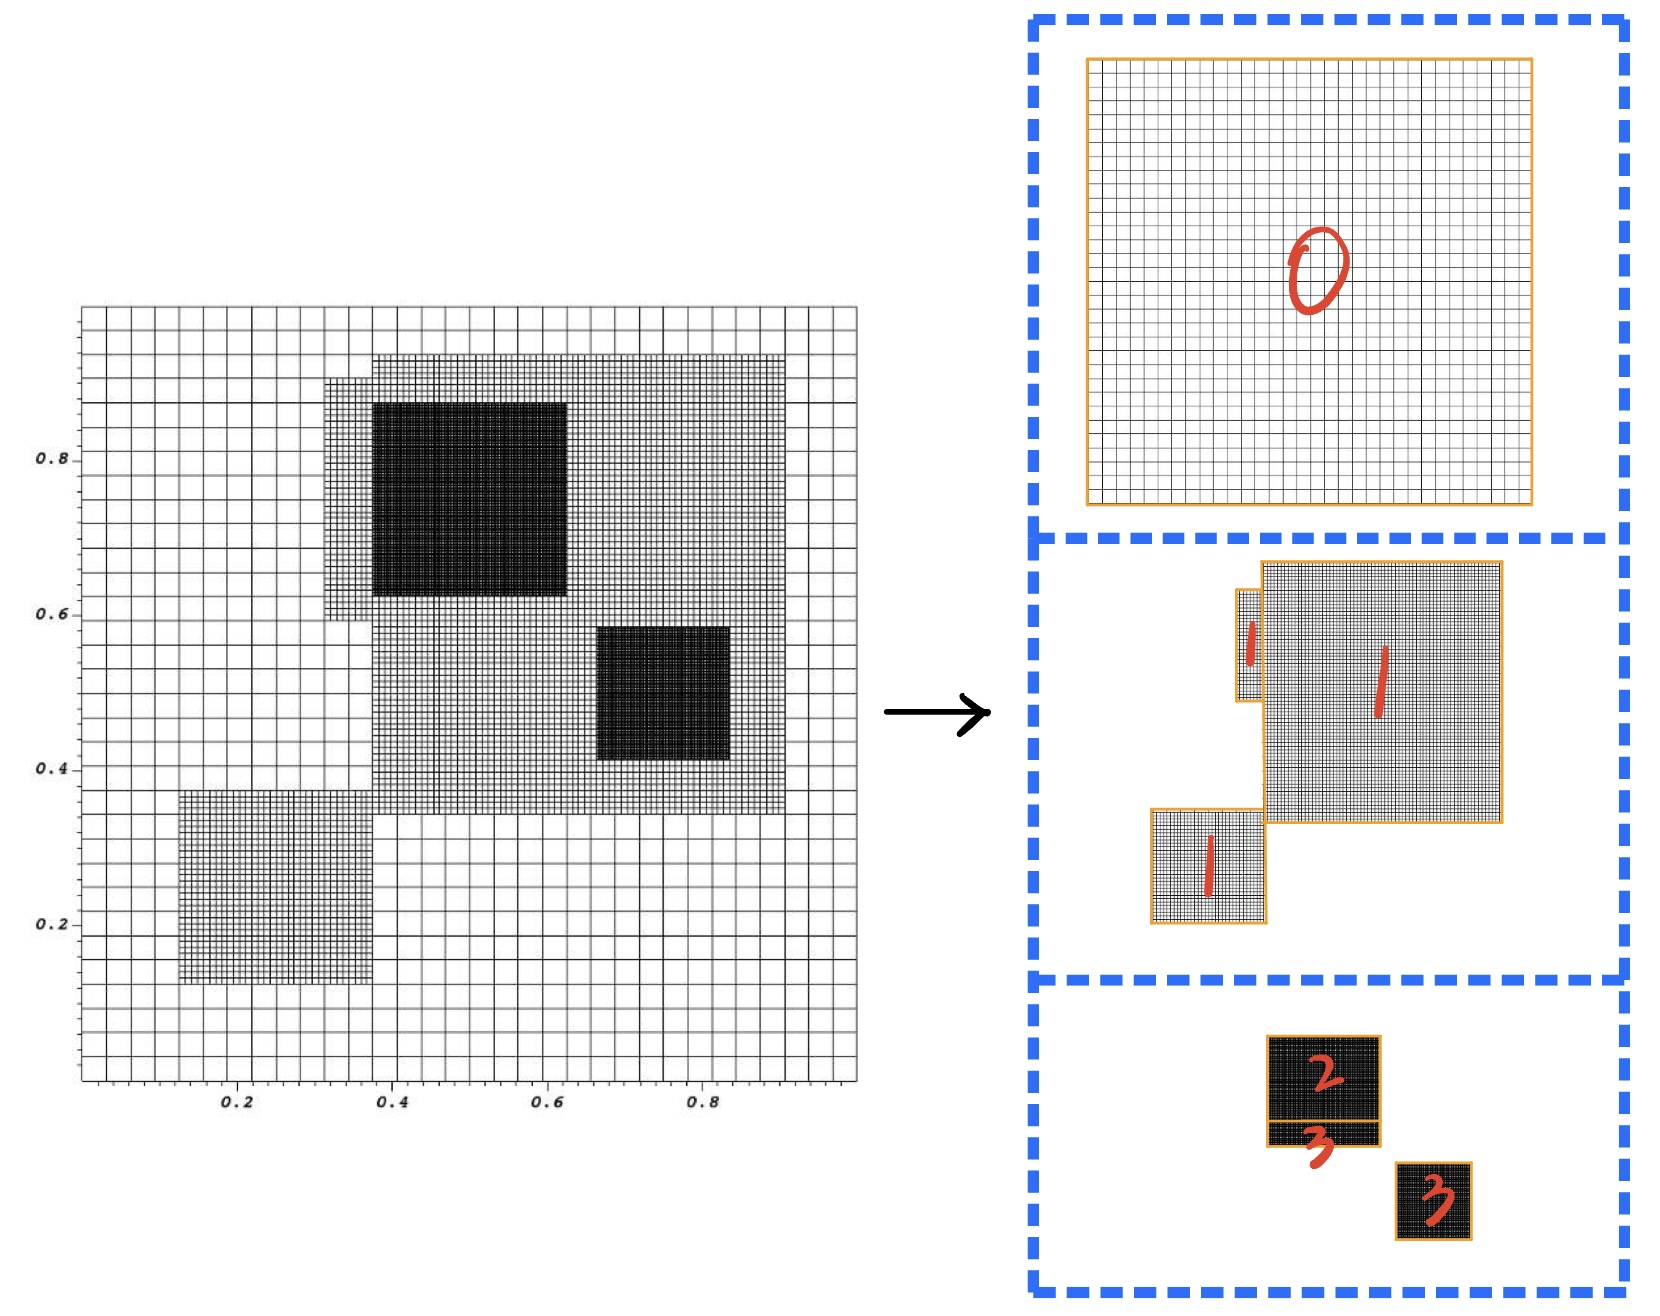
\includegraphics[width=0.65\textwidth]{jpg/newbalance.jpeg}
        \caption{\footnotesize AMR 负载均衡示意图.}
    \end{figure}
\end{frame}

\begin{frame}[fragile]{Ghost 填充器}
    \footnotesize
    物理边界的 Ghost 填充器我们已经有了, 
    我们还要填充位于区域内粗细网格交界处的 Ghost.

    \begin{figure}[H]
        \centering
        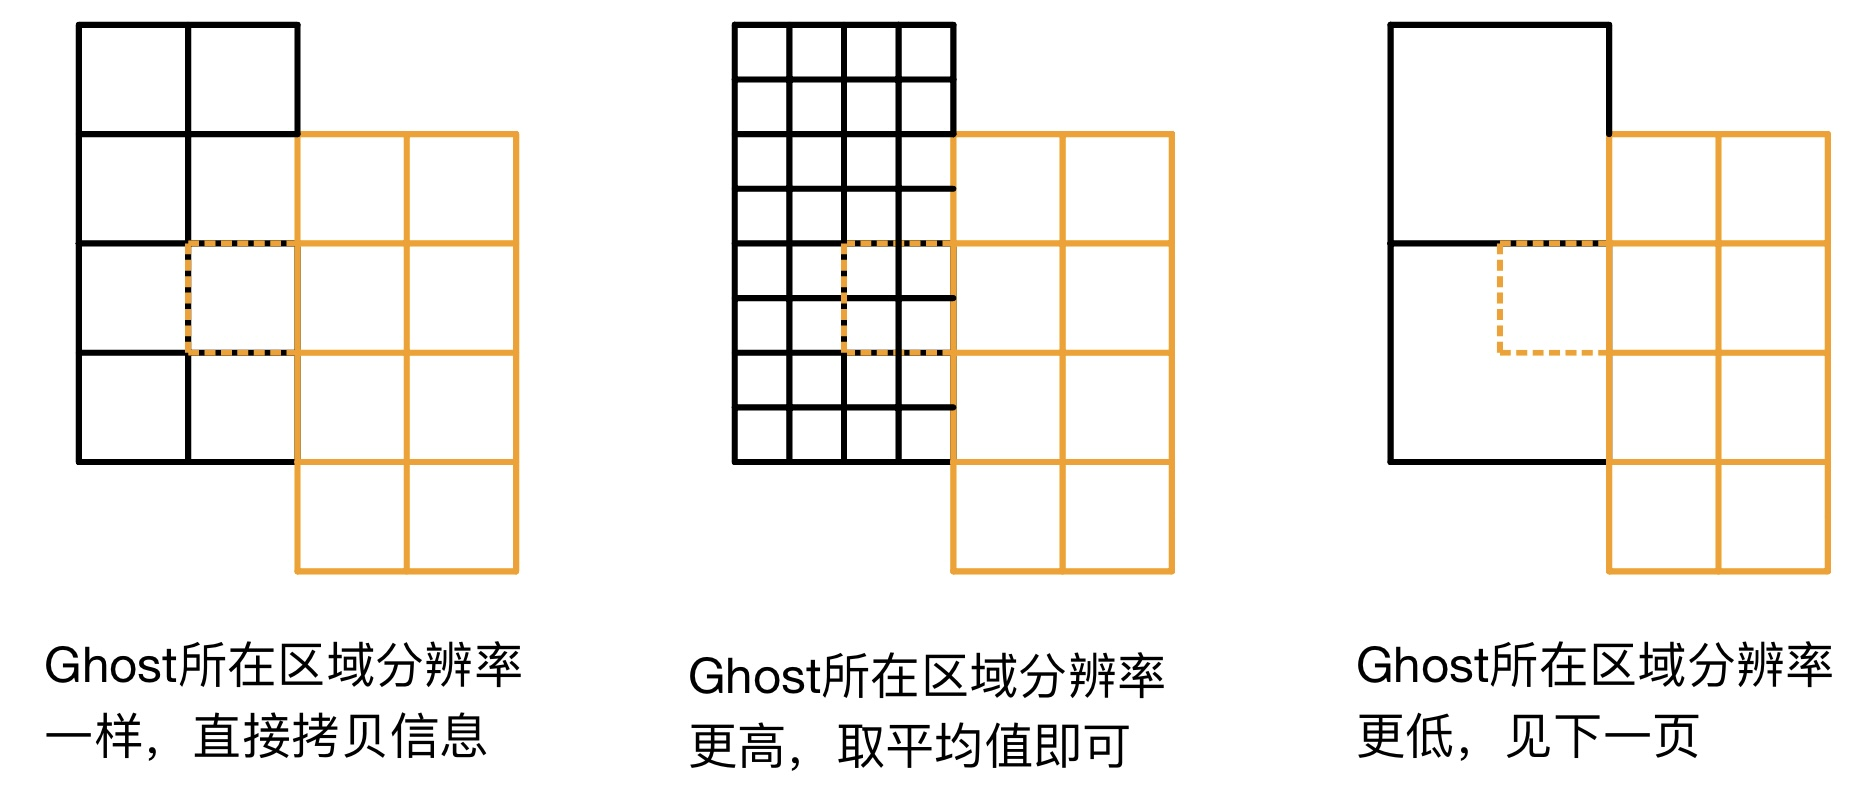
\includegraphics[width=\textwidth]{jpg/fillghost.jpeg}
        \caption{\footnotesize Ghost 填充示意图.}
    \end{figure}
\end{frame}

\begin{frame}[fragile]{Ghost 填充器}
    \footnotesize
    我们参考 Zhang 的工作\footfullcite{Zhang2011} .
    以下图所示简单的二维情形为例, 白色是粗网格区域,
    灰色是细网格区域, 对于黑色三角形所示的细网格虚拟单元,
    我们可以用圆点所示的粗网格积分平均来拟合一个四阶多项式
    (当圆点落在灰色区域内部时, 指的是对应四个细网格积分平均的平均值),
    从而计算细网格虚拟单元的取值.
    
    \begin{figure}[H]
        \centering
        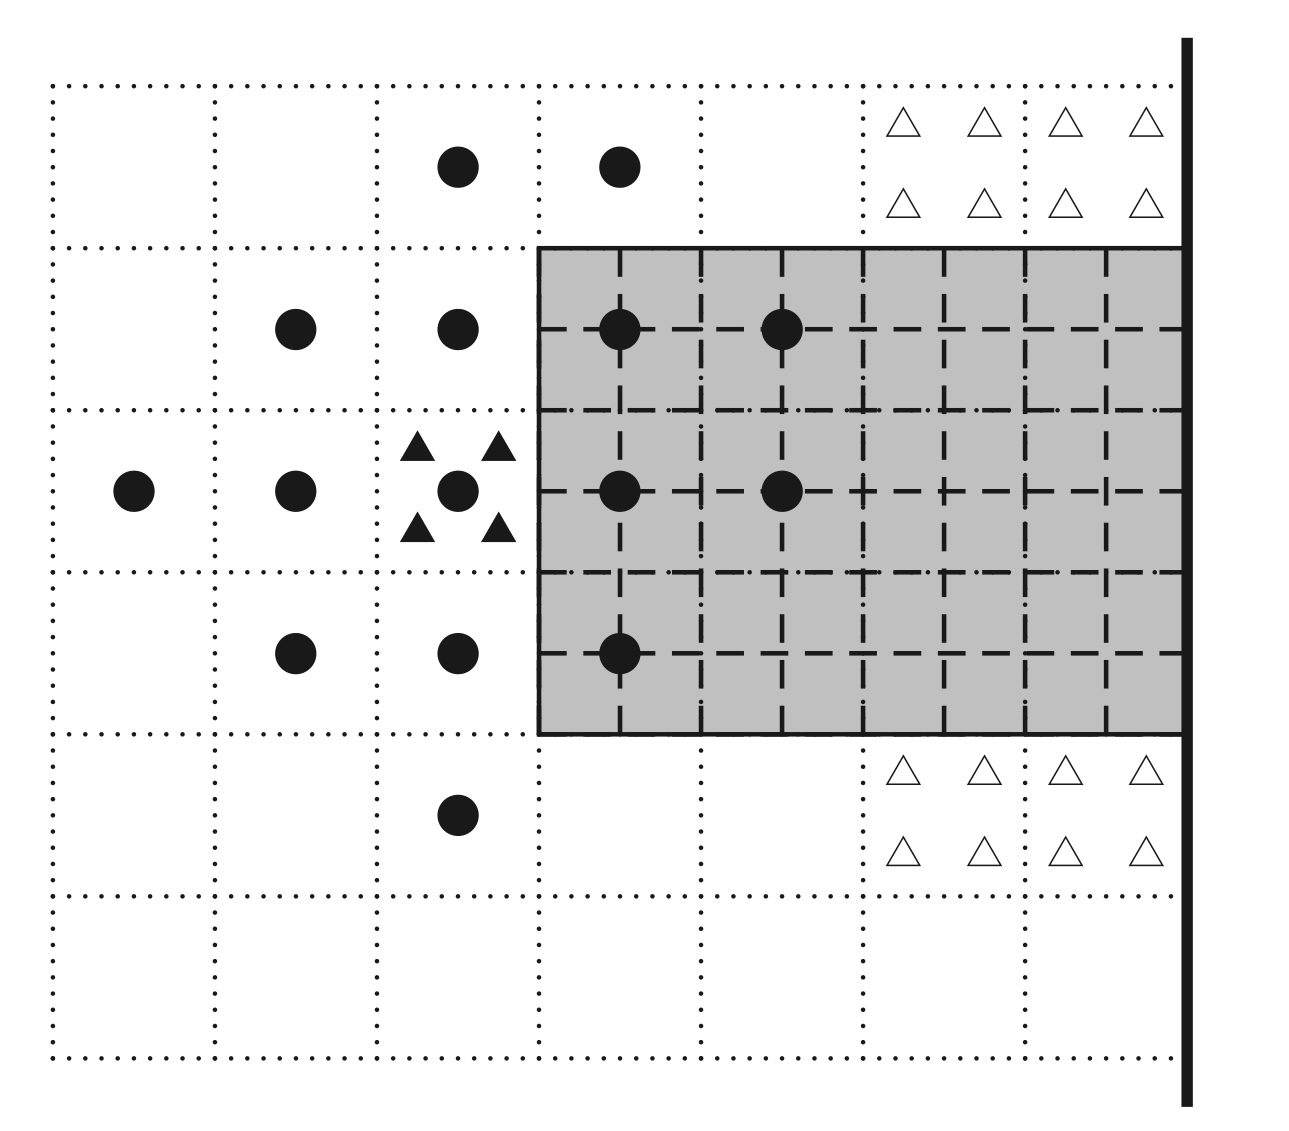
\includegraphics[width=0.4\textwidth]{jpg/fillGhost.jpeg}
        \caption{粗细网格交界处虚拟单元的填充示意图}
    \end{figure}
\end{frame}

\begin{frame}[fragile]{Ghost 填充器}
    \footnotesize
    事实上,我想把这个模块命名为 \verb|DataSwaper|.
    因为它本质是线程之间的信息交换.

    \vspace{1em}
    最主要的功能是输入一个 \verb|std::vector<LevelData>|,
    将它的 Ghost 填充好之后返回.
\end{frame}

\begin{frame}[fragile]{AMR 中的空间算子}
    \footnotesize
    首先调用 \verb|DataSwaper| 填充所有 Ghost,
    然后对每一层的 \verb|LevelData|,
    用我们现有的 \verb|SpatialOperator| 计算之.

    \begin{figure}[H]
        \centering
        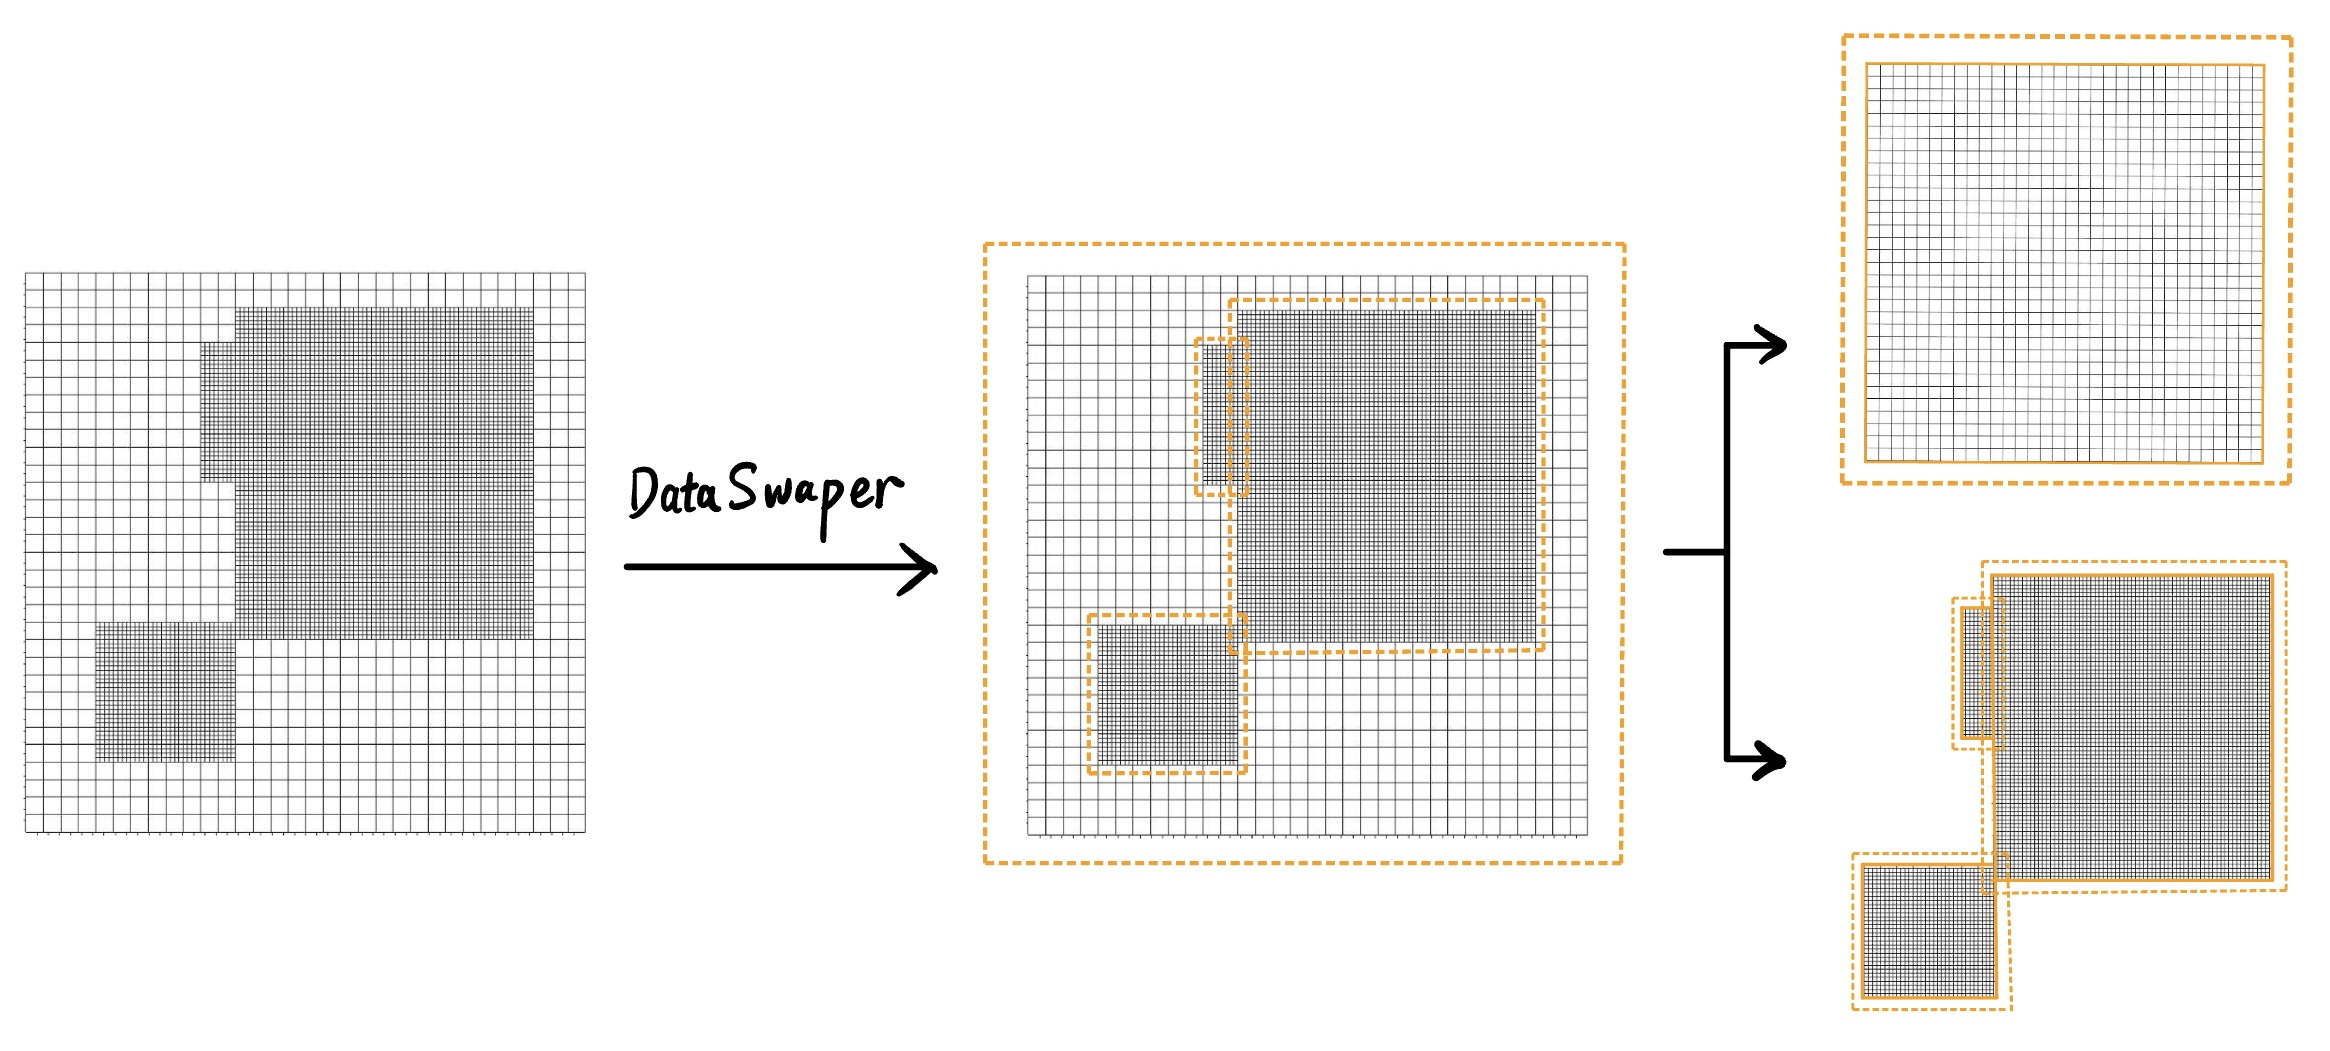
\includegraphics[width=\textwidth]{jpg/DiscOp.jpeg}
        \caption{AMR 中的空间离散算子计算示意图}
    \end{figure}

    \pause
    我想命名为 \verb|AMRSpatialOperator|,
    它的 \verb|apply|, \verb|relaxJacobi| 等函数
    的输入和输出都是 \verb|std::vector<LevelData>|.
    具体的算子类 (\verb|Diffusion|, \verb|Divergence| 等) 作为模板参数.
\end{frame}

\begin{frame}[fragile]{AMR 中的多重网格}
    \footnotesize
    改 \verb|Multigrid|, \verb|MGLevelOp|, \verb|EmHelmholtzLevelOp| 的设计.

    \begin{figure}[H]
        \centering
        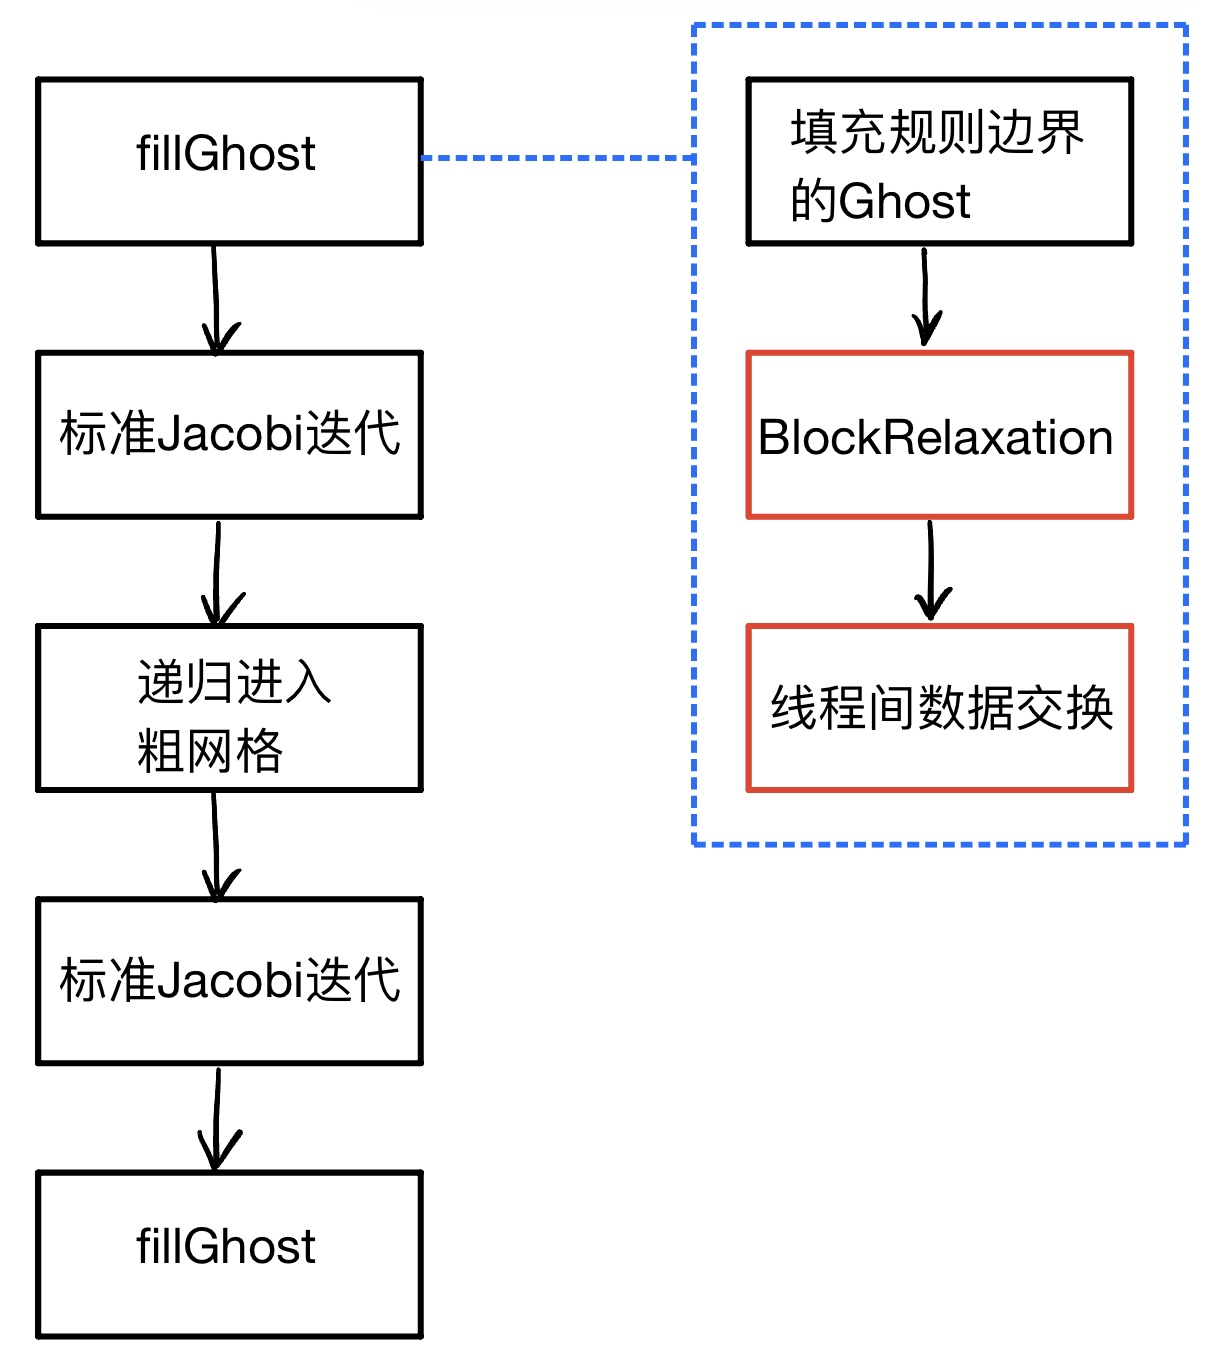
\includegraphics[width=0.4\textwidth]{jpg/amrvcycle.jpeg}
        \caption{\footnotesize AMR多重网格V-Cycle算法, 红色部分是需要大改的模块.}
    \end{figure}

    \pause
    \verb|BlockRelaxation| 我还没想好怎么改, 有两种想法:
    \begin{itemize}
        \item 直接改类的设计和实现;
        \item 我们调用原本的类, 对每层的 \verb|LevelData| 分别调用.
    \end{itemize}
\end{frame}

\begin{frame}[fragile]{AMR Poisson求解器}
    \footnotesize
    \begin{figure}[H]
        \centering
        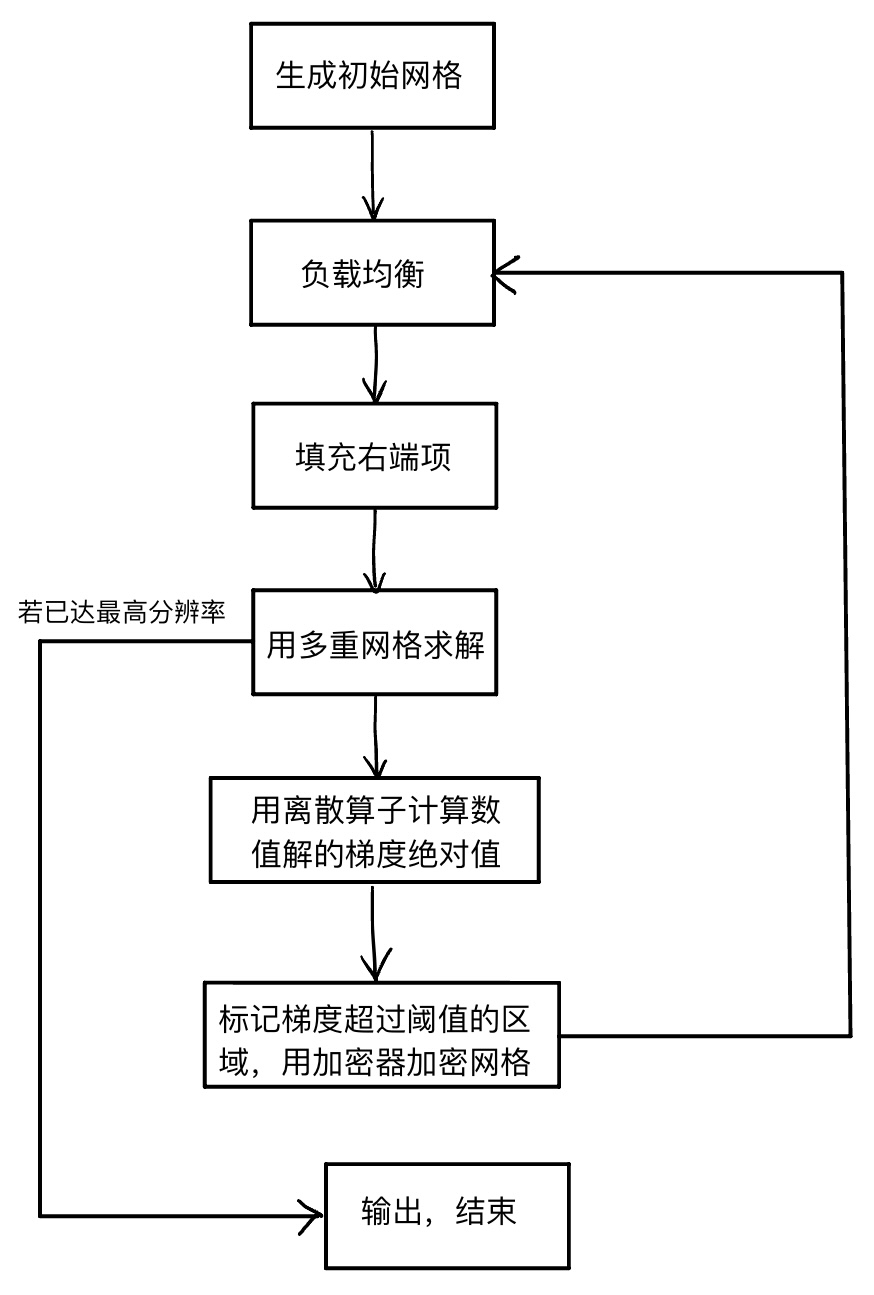
\includegraphics[width=0.4\textwidth]{jpg/poissonsolver.jpeg}
        \caption{\footnotesize AMR Poisson求解器算法流程.}
    \end{figure}
\end{frame}

\begin{frame}
    \begin{center}
        {\Huge\calligra Thank You}
    \end{center}
\end{frame}

\end{document}
